% !TeX encoding=unicode
% !TeX spellcheck = de-DE

\chapter{Basics of perturbative QCD}
\label{ch:pqcd}
The following sections give an overview of the basic principles that provide the basis for perturbative QCD.
They include the most important aspects regarding numerical calculations.
It is by far no complete depiction but it covers the parts that play a key role in the calculations used for this thesis.
%
\section{The QCD Lagrangian}
QCD is the quantum field theory that describes the strong interactions between Quarks and Gluons.
Mathematically, it is a non-abelian gauge theory with symmetry group SU(3).
Its Lagrangian is given by
%
\begin{equation}
  \Lagr_\text{QCD} = \sum_q \bar\psi_{q,a} (i \gamma^\mu \partial_\mu \delta_{ab} - g_s \gamma^\mu t_{ab}^C \glufield_\mu^C - m_q \delta_{ab}) \psi_{q,b} - \frac{1}{4} F_{\mu \nu}^A F^{A \, \mu \nu} \, ,
\end{equation}
%
where the sum goes over all quark flavors.
The $\psi_{q,a}$ are quark-field spinors, where $a=1 \dots 3$ denotes the color index, and the $\glufield_\mu^C$ are gluon fields with a color index $C=1 \dots 8$.
The strong coupling constant is denoted by $g_s$.
Quarks transform under the fundamental representation of SU(3) while gluons transform under the adjoint representation.
The $t_{ab}^C$ are  the generators of the group.
The gluon field tensor $F_{\mu \nu}^A$ is given by
%
\begin{equation}
	F_{\mu \nu}^A = \partial_\mu \glufield_\nu^A - \partial_\nu \glufield_\mu^A - g_s f_{ABC} \glufield_\mu^B \glufield_\nu^C \, ,
\end{equation}
%
where the $f_{ABC}$ are the structure constants of the group, defined through $[ t^A,t^B ] = i f_{ABC} t^C$.
In comparison to quantum electrodynamics (QED), the main difference is the presence of the interaction term $- g_s f_{ABC} \glufield_\mu^B \glufield_\nu^C$ which results in the existence of 3-gluon and 4-gluon vertices.

The perturbative approach to QCD is to write the observables as a power series in $\alpha_s = g_s^2/(4 \pi)$:
%
\begin{equation}
  F = F^{(1)} \alpha_s + F^{(2)} \alpha_s^2 + \dots \, ,
\end{equation}
%
where $\alpha_s \ll 1$ so that the series can be truncated after a few terms to obtain a useful approximation.
This leads to leading order (LO), next-to-leading order (NLO), next-to-next-to-leading order (NNLO)\ldots{} predictions.
A straightforward way to determine the coefficients is the use of Feynman Diagrams.
%
\section{Renormalization and the running coupling}
Calculations in perturbative QCD involve UV-divergent integrals.
Luckily QCD is a renormalizable theory and therefore the divergences can be handled by regularization and renormalization.
As a consequence, the quantities appearing in the Lagrangian (the \enquote{bare} quantities) are not the same as the quantities that are physically observed.
In the renormalization process, an additional scale dependence is introduced which vanishes if we consider the whole perturbative series.
The evolution of quantities with the renormalization scale $\mu_R$ is described by differential equations known as \textit{renormalization group equations}.
As an example, the \enquote{running} of the coupling constant is described by
%
\begin{equation}
  \dod{ \alpha_{s} ( \mu_R^{2} ) }{ \ln{\mu_R^2} } = \beta(\alpha_s(\mu_R^2)) = - \alpha_s^2 (b_0 + b_1 \alpha_s + b_2 \alpha_s^2 + \dots) \, .
	\label{eq:rge}
\end{equation}
%
The minus sign in \cref{eq:rge} is responsible for the asymptotic freedom of QCD:
As the momentum transfer becomes large, the strong coupling becomes weak so that quarks and gluons nearly behave as if they were free particles.

In leading order the analytic solution of \cref{eq:rge} is given by
%
\begin{equation}
	\alpha_s(\mu_R^2) = \frac{\alpha_s(\mu_0^2)}{1 + b_0 \alpha_s(\mu_0^2) \ln \frac{\mu_R^2}{\mu_0^2}} \quad \text{with} \quad b_0=\frac{11 N_C - 2 n_f}{12 \pi} \, ,
\end{equation}
%
where $N_C$ is the number of colors and $n_f$ denotes the number of active flavors.
This relates the coupling constant at a scale $\mu_R$ to the one at a reference scale $\mu_0$, where its value is known.
%
\section{From parton model to QCD}
The parton model was introduced in 1969 by Richard P. Feynman to describe high-energy particle collisions involving hadrons \cite{feynman1969}.
The basic assumption of the parton model is that all hadrons consist of point-like spin-$\frac{1}{2}$ particles (partons) which are responsible for their behavior in interactions.
%In QCD these can be identified as quarks and gluons.
Furthermore, it is assumed that the hadron is in a reference frame where it carries infinite (or at least very high) momentum.
In this infinite momentum frame the hadron suffers both Lorentz contraction and time dilation so that the distribution of partons within it does not change during the (vanishingly small) time of interaction.
Thus each parton carries a definite fractional momentum $x$, with $0<x<1$.
In addition, the process of hadronization due to quark confinement happens too late to influence the interaction.
Another important consequence is that the probability of a parton influencing the scattering of another parton is suppressed (\enquote{incoherence} of the parton model).
The reason this model works is the asymptotic freedom of the underlying theory.
However, this also limits the applicability of the parton model to high energy cross sections.

By itself, the parton model does not make any assumptions about the distribtion of partons inside the hadron.
It just introduces it as a parameter in the form of \textit{parton distribution functions} (PDFs) $f_i(x)$, which represent the probability of finding a parton of type $i$ carrying a momentum fraction $x$ of the hadron.
As they cannot be derived from first principles they have to be extracted from measured data.
This is the task of different PDF fitting groups like HERAPDF \cite{herapdf}, CTEQ \cite{ct10}, MSTW \cite{mstw2008} and NNPDF \cite{nnpdf1}.
Parton model predictions then take the form of a convolution of the parton level interaction with the PDF, summarized over all possible parton flavors.
We call this the \enquote{naive} parton model.

The naive parton model works well as long as the energy scale is not too high.
Otherwise we need to include higher order corrections which can arise from real emissions and virtual loops.
These involve infrared divergencies that cancel each other exactly thanks to the Kinoshita–Lee–Nauenberg theorem \cite{kln_theorem1,kln_theorem2}, rendering perturbative QCD as a whole an infrared safe theory.
However, the cancellation is not guaranteed if we truncate the perturbative series after a finite number of terms.
In processes involving initial-state hadrons, the partons can emit gluons before entering the hard interaction (see \cref{fig:initial_gluon}).%
%
\begin{figure}
\centering
	\begin{subfigure}[]{0.3\textwidth}
		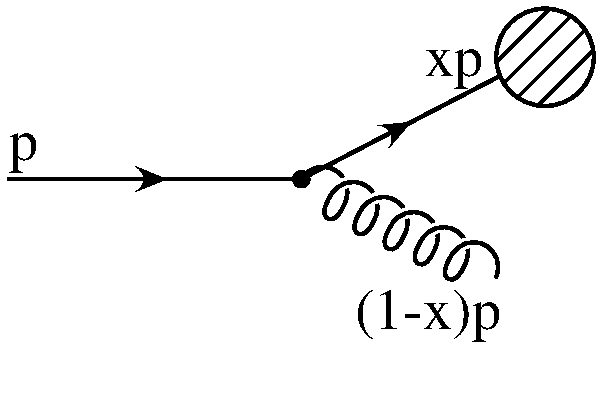
\includegraphics[width=\textwidth]{images/initial_real.pdf}
	\end{subfigure}
	\hspace{1cm}
	\begin{subfigure}[]{0.3\textwidth}
		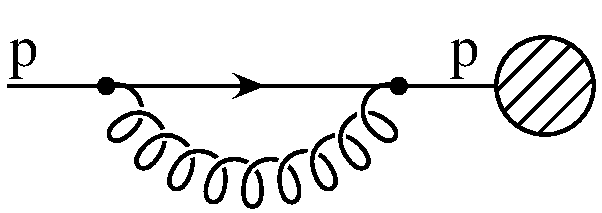
\includegraphics[width=\textwidth]{images/initial_virtual.pdf}
	\end{subfigure}
	\caption{Feynman diagrams for initial-state gluon emission.}
	\label{fig:initial_gluon}
\end{figure}
%
However, there is an important difference between real and virtual emissions in this case:
While the virtual emission does not change the momentum of the parton entering the process, the real gluon carries off parts of the parton momentum.
Thus, the total cross section consists of two different hard cross sections that do not cancel in the collinear limit.
This is a consequence of the collinear limit corresponding to long-range effects of the strong interaction, which are not calculable in perturbation theory.

In order to be able to calculate cross sections with initial-state hadrons, we can take a similar approach as for the renormalization of the coupling constant and introduce a scale variable which we call the \textit{factorization scale} $\mu_F$.
All the non-perturbative parts are cut off at $\mu_F$ and absorbed into the PDF.
There is an arbitrariness in how much of the correction terms is to be factored out.
This is defined by the \textit{factorization scheme}.
Common schemes include the DIS scheme, in which all non-leading order contributions are absorbed into the PDFs, and the $\overline{MS}$ scheme, in which only the divergent parts are absorbed.
Once the factorization scheme has been chosen, it has to be used consistently in all following cross section calculations.

As an example, let us consider the cross section for a scattering process involving two initial state hadrons $h$ and $h'$ with momenta $p$ and $p'$, which now takes the factorized form
%
\begin{equation}
	\sigma_{h,h'} = \sum_{i,j} \int \dif x \dif x' f_{i/h}(x,\mu^2) \cdot \sigma_{ij}(x p,x' p',\alpha_s(\mu^2)) \cdot f_{j/h'}(x',\mu^2) \, ,
	\label{eq:hadron_crosssection}
\end{equation}
%
where we have taken $\mu_R = \mu_F= \mu$ and where the sum includes all possible initial state parton combinations.
$\sigma_{ij}$ denotes the hard parton-level cross section which can be calculated in perturbation theory.
All the non-perturbative long-distance contributions are factorized into the PDFs.
%
\section{DGLAP evolution}
Analogous to the running coupling, we can define a renormalization group equation that describes the evolution of the PDFs with the factorization scale.
It is called the Dokshitzer-Gribov-Lipatov-Altarelli-Parisi (DGLAP) equation \cite{dglap1,dglap2,dglap3} and takes the form of a matrix equation spanning all quark flavors and the gluon:
%
\begin{align}
	\dod{}{\ln{\mu_F^2}} \begin{pmatrix} q_i(x,\mu_F^2) \\ g(x,\mu_F^2) \end{pmatrix} = &\frac{\alpha_s(\mu_F^2)}{2 \pi} \sum_{q_j,\bar q_j} \int_x^1 \frac{\dif z}{z} \nonumber \\
	&\cdot \begin{pmatrix}
		P_{q_i q_j}(\frac{x}{z},\alpha_s(\mu_F^2))	&	P_{q_i g}(\frac{x}{z},\alpha_s(\mu_F^2)) \\
		P_{g q_j}(\frac{x}{z},\alpha_s(\mu_F^2))	&	P_{gg}(\frac{x}{z},\alpha_s(\mu_F^2))
	\end{pmatrix}
	\begin{pmatrix} q_j(z,\mu_F^2) \\ g(z,\mu_F^2) \end{pmatrix} \, .
	\label{eq:dglap}
\end{align}
%
The $P_{i j}(x,\alpha_s)$ are called splitting functions and they imply the probability of a parton splitting into two other partons.
They are calculable in perturbation theory and are known up to NNLO \cite{splittingkernel1,splittingkernel2}.
The DGLAP equation allows to evolve the PDFs from an initial scale $Q_0$ to another scale $Q$ without further knowledge and thus is one of the most important equations of perturbative QCD.
%
\section{Next-to-leading order calculations}
\label{sec:nlo_calculations}
When going from LO calculations at tree level to NLO, one has to take into account real emissions from the colored particles and virtual loops.
In general, both the real and the virtual corrections are seperately divergent and need to be regularized.
There are two general methods that are commonly used to take care of the infrared divergences in NLO calculations, namely the \textit{slicing method} and the \textit{subtraction method}.
The slicing method introduces a small parameter $\delta$, which slices the integration region into two pieces so that it can be computed numerically.
A residual dependency on $\delta$ remains, which should be neglectable if $\delta$ is small.
However, this has to be checked in an actual calculation.
The advantage of the subtraction method is that it does not involve any approximations.

We can demonstrate the subtraction method with a simple example, that has been adopted from \cite{mcatnlo}.
Consider the expression for the expectation value of an infrared-safe observable $O$ at NLO accuracy, consisting of a Born (B), a virtual (V) und a real (R) term:
%
\begin{equation}
	\left< O \right> = \lim_{\epsilon \rightarrow 0} \int_0^1 \dif x x^{-2 \epsilon} O(x) \left[ \left( \od{\sigma}{x} \right)_B + \left( \od{\sigma}{x} \right)_V + \left( \od{\sigma}{x} \right)_R \right] \, .
\end{equation}
%
We assume that the cross sections can be written as
%
\begin{align}
	\left( \od{\sigma}{x} \right)_B &= B \delta(x) \, , \\
	\left( \od{\sigma}{x} \right)_V &= a \left( \frac{B}{2 \epsilon} + V \right) \delta(x) \, , \\
	\left( \od{\sigma}{x} \right)_R &= a \frac{R(x)}{x} \, ,
\end{align}
%
where $B$ and $V$ are constant factors and $\lim_{x \rightarrow 0} R(x) = B$.
$a$ denotes the coupling constant.
Obviously, both the real and the virtual part are divergent in the limit $\epsilon \rightarrow 0$.
Using the subtraction method, we can rewrite the real contribution to obtain
%
\begin{align}
	\left< O \right>_R	&= a \lim_{\epsilon \rightarrow 0} \int_0^1 \frac{\dif x}{x^{1+2 \epsilon}} O(x) R(x) \nonumber \\
						&= a B O(0) \lim_{\epsilon \rightarrow 0} \int_0^1 \frac{\dif x}{x^{1+2 \epsilon}} + a \int_0^1 \frac{\dif x}{x} [O(x) R(x) - B O(0)] \nonumber \\
						&= -a B O(0) \lim_{\epsilon \rightarrow 0} \frac{1}{2 \epsilon} + a \int_0^1 \frac{\dif x}{x} [O(x) R(x) - B O(0)] \, .
	\label{eq:toymodel_realsub}
\end{align}
%
By explicitely writing down the virtual part,
%
\begin{equation}
	\left< o \right>_V = a \lim_{\epsilon \rightarrow 0} \int_0^1 \frac{\dif x}{x^{2 \epsilon}} O(x) \left( \frac{B}{2 \epsilon} + V \right) \delta(x) \, ,
\end{equation}
%
we see that the first term gets exactly cancelled by the first term on the right hand side of \cref{eq:toymodel_realsub}.
Including the Born contribution we arrive at the expression
%
\begin{equation}
	\left< O \right> = B O(0) + a \left\{ V O(0) + \int_0^1 \frac{\dif x}{x} [O(x) R(x) - B O(0)] \right\} \, ,
\end{equation}
%
which now only consists of finite terms.
The remaining integral can be evaluated using Monte Carlo methods.
The subtraction method can be generalized to arbitrary hadronic cross sections, provided that the definition of the observables allows the cancellation of the divergences.
%
\section{Parton showers}
There are phase space regions that cannot be well described by fixed order calculations in perturbation theory.
These include collinear parton splitting and soft gluon emission, which are closely related to the presence of infrared divergences.
To describe them accurately, higher order terms need to be considered.
However, the work required to derive the needed matrix elements quickly increases with each order, which is the reason why most processes have not been calculated further than NLO.
We need a different approach to deal with the problematic phase space regions.
Instead of relying on a fixed order calculation, we can consider an approximate model that includes the dominant contributions at all orders.
In this model, the collinear splitting and soft gluon emission of every parton in the initial and final state is simulated with respect to the related probabilities.
The additional partons are again able to split or radiate gluons.
By recursively applying this procedure, we obtain a cascade of parton emissions, called a \textit{parton shower}.
An example is illustrated in \cref{fig:partonshower}.
The shower ends when a certain cut-off scale is reached.
%
\begin{figure}[]
	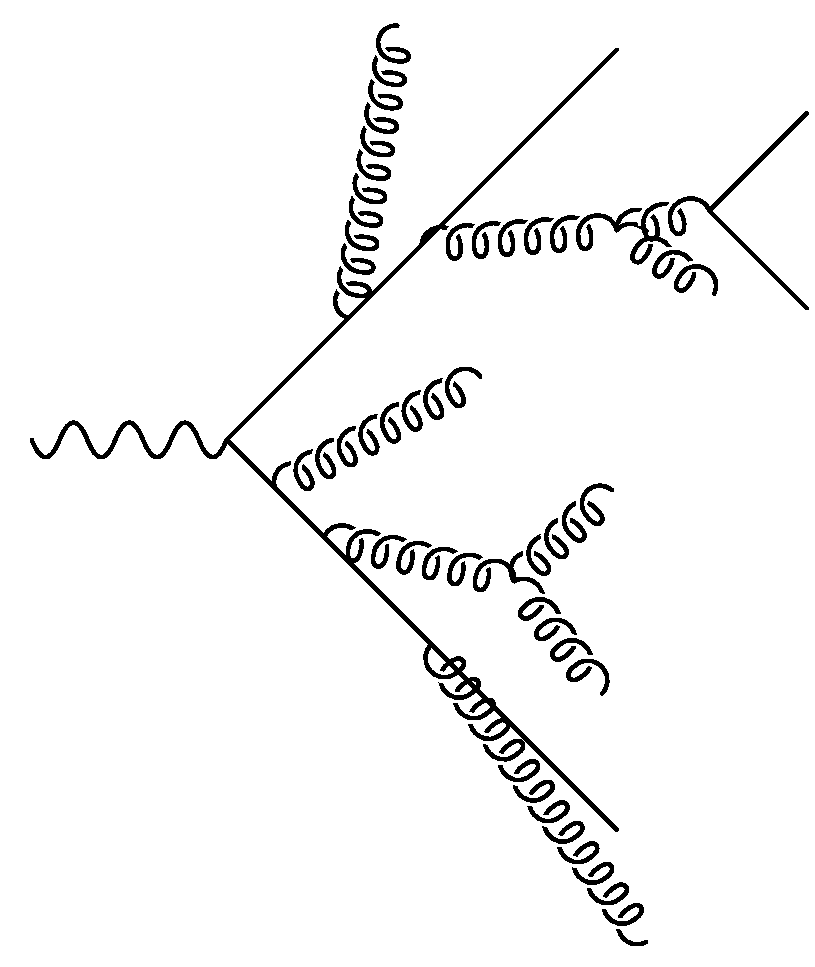
\includegraphics[width=0.5\textwidth]{images/partonshower.pdf}
	\caption{Example of a parton shower.}
	\label{fig:partonshower}
\end{figure}
%

The evolution of the splitting with the decreasing scale is given by the DGLAP equation \cref{eq:dglap}.
In this context the PDFs do not describe the momentum distributions of the partons inside of a hadron, but rather the distribution of the momentum fractions of the partons resulting from the splitting.

The computation of parton showers can be formulated in a way that is well suited for a Monte Carlo program.
We can combine the parton shower program with a hadronization model, that combines both the initial state and the final state partons into colorless hadrons, beginning at the cutoff scale of the shower. We call the result a \textit{parton shower Monte Carlo event generator}.
It is a powerful tool that is able to fully simulate QCD events in hadron collisions.

The main disadvantage of parton shower generators is that they are not guaranteed to properly describe events that include hard and large-angle emissions.
Those events are, however, correctly described by fixed order calculations.
To combine the benefits of both, algorithms have been developed that merge LO matrix elements and parton showers with different multiplicities (MEPS).
The main issue in the course of this is double counting.
An event with $n$ partons in the final state can either be the product of an $n$-parton matrix element that has been showered with only soft and collinear emissions or it could be the product of an $(n-1)$-parton matrix element for which the showering led to the emission of a hard, large-angle gluon.
Those cases have to be carefully seperated to avoid an overrepresentation of the related phase space region.
The most widely used methods to avoid double counting are CKKW matching \cite{ckkw_a,ckkw_b} and MLM matching \cite{mlm_a,mlm_b}.

Another problem of parton shower predictions is that they suffer from strong scale dependence because they are based on LO matrix elements.
Promoting parton showers to NLO accuracy is a much harder task because of divergent event weights.
Nonetheless, there are methods to circumvent this problem and the two widely used solutions are \mcatnlo{} \cite{mcatnlo} and \powheg{} \cite{powheg_a,powheg_b,powheg_c}.
As of recently, it is also possible to merge different jet multiplicities in NLO calculations matched to parton showers \cite{nlomerging1,nlomerging2,nlomerging3,nlomerging4,nlomerging5}.

